\documentclass[11pt]{article}
\usepackage{fullpage}
\usepackage{fancyhdr}
\usepackage{enumerate}
\usepackage{graphicx}
\usepackage{amsmath}

\renewcommand{\maketitle}{
  \begin{center}
    \begin{flushright}
      Dan Friedman \& Peter Fogg \\
      CSCI 343 \\
      HW4 -- TCP SYN flood
    \end{flushright}
    \rule{\linewidth}{0.1mm}
  \end{center}
}

\begin{document}
\maketitle
\begin{enumerate}
\item To begin a TCP connection, the client sends a SYN message to the server. The server acknowledges with a SYN-ACK, which is received by the client, who then responds with an ACK. This is known as the three-way handshake. To create a SYN flood, the attacking client sends SYN packets but never responds to the SYN-ACK. The server will wait for the ACK, using some resources to maintain state. With enough SYN messages, the server runs out of resources -- in particular, it must maintain the state of each connection in the SYN queue. Once this queue is filled by the half-open connections to the attacker, the server cannot serve new (legitimate) requests.
\item TCP sequence numbers are chosen arbitrarily by the server. This allows us to encode some information, if we want. A SYN cookie encodes the state of the connection, which otherwise would have been stored in the SYN queue. This removes the need for the queue, and so a SYN flood attack cannot use up server resources.
\item \text{}
  \begin{center}
    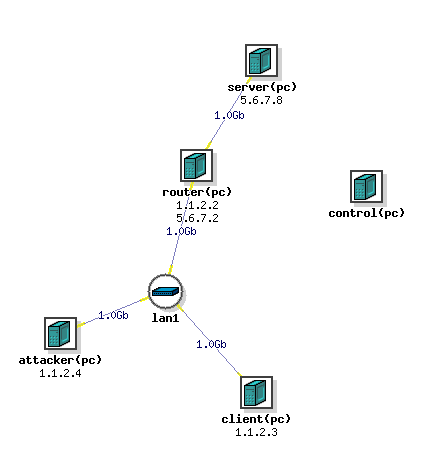
\includegraphics[width=3.5in]{topology.png}
  \end{center}
\newpage
\item \text{}
  \begin{center}
    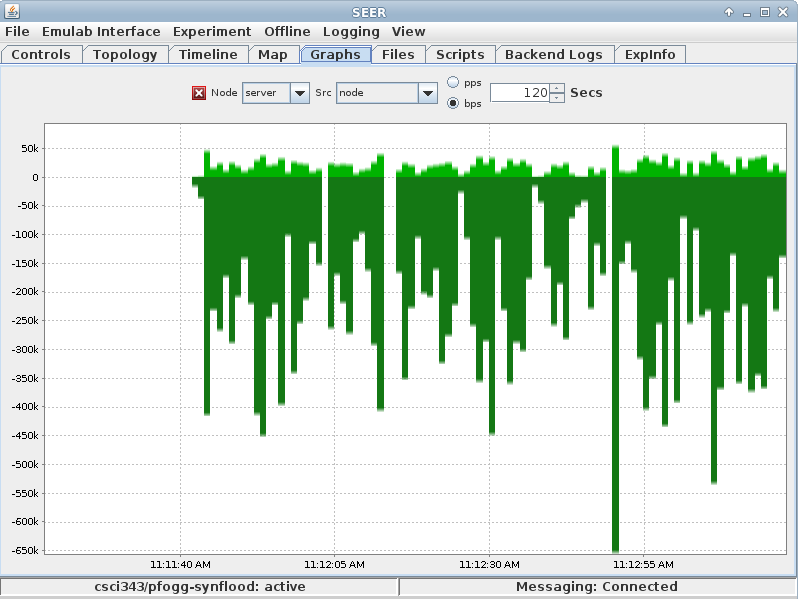
\includegraphics[width=3.5in]{green-traffic.png}
  \end{center}
\item \text{}
  \begin{center}
    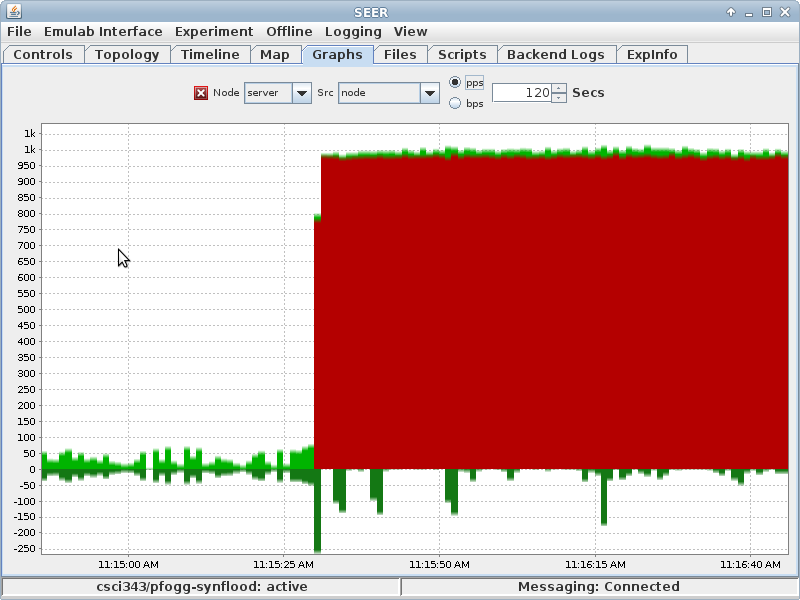
\includegraphics[width=3.5in]{red-traffic.png}
  \end{center}
  The attacker is sending SYNs with a spoofed IP address, in order to look like the client. So the server's ACK messages are all going to the client, which looks like legitimate traffic.
\newpage
\item \text{}
  In the following two graphs, each dot represents a connection.  The x-axis indicates the time at which each connection was initiated, while the y-axis represents the duration of the connection.
  \begin{center}
    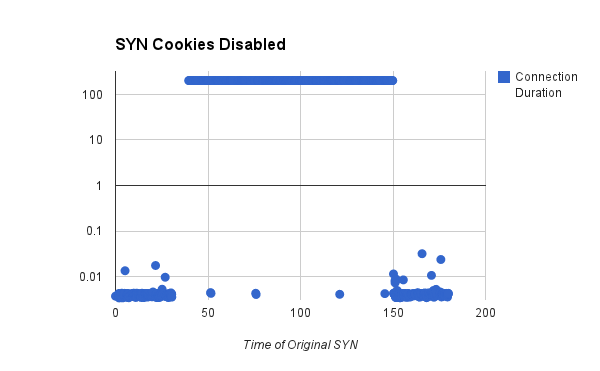
\includegraphics[width=3.5in]{without-cookies.png} \\
  \end{center}
  When SYN cookies weren't enabled (above graph), we saw that connections consistently timed out for the extent of the attack, which started at the 30 second mark and ended at 150 seconds.  Only about four connections did \emph{not} time out during the SYN flood.  Since almost all traffic timed out in this way, this instance of the SYN flood attack is an effective denial of service.  \emph{Note: we scaled the y-axis logarithmically in this graph to show more detail before/after the attack}
  \begin{center}
    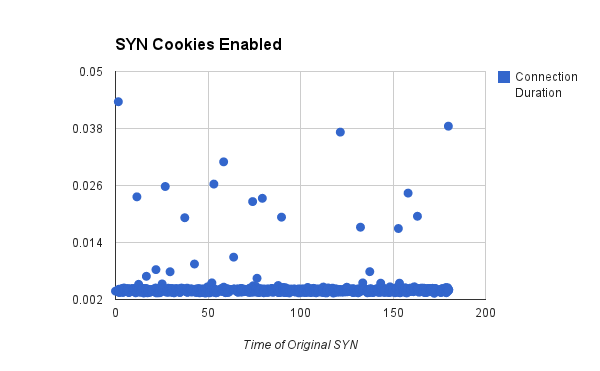
\includegraphics[width=3.5in]{with-cookies.png}
  \end{center}
  Once SYN cookies were enabled, connection durations remained consistent during the attack (above graph).  Higher dots correspond to longer connection times, but the dots are not raised in the 30-150 second range.  Most importantly, not even one connection timed out!  We conclude that SYN cookies are an effective defence against a SYN flood.
\end{enumerate}
\emph{We affirm that we have adhered to the Honor Code in this assignment.}
\end{document}
